\documentclass[12pt]{article}
\usepackage{graphicx} % Required for inserting images
\usepackage[a4paper, inner= 1.5in, outer= 1in, top= 1in, bottom= 1in]{geometry}
\usepackage[onehalfspacing]{setspace} % to create a half spacing of 1.5 in
% \thispagestyle{}
\usepackage{ragged2e}
\usepackage{times}
\usepackage{fancyhdr}
\usepackage{url}

\fancyhf{}
\pagenumbering{arabic}



\newcommand{\theinstitute}{Institute of Engineering}
\newcommand{\thecampus}{Lalitpur Engineering College}
\newcommand{\thedepartment}{Department of Computer Engineering}
\newcommand{\thedepartmentAddress}{Kathmandu, Nepal}
\newcommand{\thedepartmentFullAddress}{Chakupat, Lalitpur, Nepal}
\newcommand{\theprogramcoordinator}{Er. Bisikha Subedi}
\newcommand{\theHOD}{Er. Praches Acharya}
\newcommand{\thesupervisor}{Er. Bishika Subedi}



\newcommand{\thetitle}{DefaceLab:  DeepFake Detection using Deep Learning}
\newcommand{\theauthor}{ABHISHEK NEUPANE [LEC076BCT002]
    \\RABINDRA ADHIKARI [LEC076BCT025]
    \\SANJISH MAHARJAN [LEC076BCT032]
    \\SUSHIL KAFLE [LEC076BCT045]}


\begin{document}


\begin{center}

    \thispagestyle{empty}
    {\fontsize{16 pt}{12} \selectfont\textbf{TRIBHUVAN UNIVERSITY} \\
        \textbf{INSTITUTE OF ENGINEERING}} \\
    \vspace{0.3 in}

    
\includegraphics[width= 3in ]{img/leclogo21.png} \\
    \vspace{0.05 in}
    LALITPUR ENGINEERING COLLEGE \\
    CHAKUPAT, LALITPUR \\

    \vspace{0.5 in}
    \textbf{ A PROPOSAL OF MAJOR PROJECT}\\
    {\fontsize{16 pt}{12} \selectfont \textbf{\thetitle}}\\
    \vspace{1.1 in}
    \textbf{ SUBMITTED BY}  \\
    {\theauthor} \\
    \vspace{1.1 in}
    \textbf{ SUBMITTED TO}  \\
    DEPARTMENT OF COMPUTER ENGINERING \\
    \vspace{1 in}
    \textbf{Bhadra 2080} \\
\end{center}
\begin{center}
    \linespread{1.6}
    \thispagestyle{empty}
    
\includegraphics[width= 3in ]{img/leclogo21.png} \\
    \vspace{0.05 in}
    {\fontsize{12 pt}{12} \selectfont\textbf{TRIBHUVAN UNIVERSITY} \\
        \textbf{INSTITUTE OF ENGINEERING} \\
        % \vspace{0.3 in}
        \textbf{LALITPUR ENGINEERING COLLEGE}} \\
    % CHAKUPAT, LALITPUR} \\

    \vspace{0.5 in}
    \textbf{A project Report}\\
    {\fontsize{12 pt}{12} \selectfont\textbf{On}\\}
    {\fontsize{12 pt}{12} \selectfont \textbf{\thetitle}}\\
    \vspace{0.4 in}
    \textbf{ Submitted By:}  \\
    {\theauthor} \\
    \vspace{0.3 in}
    \textbf{ Submitted To:}  \\
    Department of Computer Engineering \\
    Lalitpur Engineering College \\
    Chakupat, Lalitpur \\

    \vspace{0.2in}
    In partial fulfillment for the award of the
    Bachelor's Degree in Computer Engineering

    \vspace{0.2in}
    \textbf{Under the Supervision of} \\
    \thesupervisor\\
    \vspace{0.2in}
    \thedate

\end{center}


\newpage

\begin{center}
    
    
    \pagenumbering{Roman}
    \section*{ABSTRACT}
    \justify
    Deepfakes are realistic-looking fake media generated by deep-learning algorithms that iterate through large datasets until
    they have learned how to solve the given problem (i.e., swap faces or objects in video and digital content). The massive generation
    of such content and modification technologies is rapidly affecting the quality of public discourse and the safeguarding of
    human rights. Deepfakes are being widely used as a malicious source of misinformation in court that seek to sway a court’s decision.
    Because digital evidence is critical to the outcome of many legal cases, detecting deepfake media is extremely important and in high demand in digital forensics.
    As such, it is important to identify and build a classifier that can accurately distinguish between authentic and disguised media, especially in facial-recognition systems
    as it can be used in identity protection too. In this work, we compare the most common, state-of-the-art face-detection classifiers such as Custom CNN, VGG19, and DenseNet-121
    using an augmented real and fake face-detection dataset. Data augmentation is used to boost performance and reduce computational resources. Our preliminary results indicate that VGG19 has the best performance
    and highest accuracy of 95\% when compared with other analyzed models.\\
    \vspace{3 in}
    \\ \textit{Keywords: deepfake detection; digital forensics; media forensics; deep learning; VGG19; face-image manipulation}
    
    
\end{center}
\newpage


\tableofcontents
\thispagestyle{empty}
\newpage
\listoffigures
\newpage
\section*{List of Abbreviations}
\begin{table}[h]

    \renewcommand{\arraystretch}{1.5}
    \begin{tabular}{@{}p{0.3\linewidth}p{0.6\linewidth}@{}}
        AUC     & Area Under the Curve              \\
        CNN     & Convolutional Neural Network      \\
        DFD     & Data Flow Diagram                 \\
        ELU     & Exponential Linear Unit           \\
        FN      & False Negative                    \\
        FP      & False Positive                    \\
        FPR     & False Positive Rate               \\
        FPS     & Frames Per Second                 \\
        GANs    & Generative Adversarial Networks   \\
        GELU    & Gaussian Error Linear Unit        \\
        JWT     & JSON Web Token                    \\
        KDE     & Kernel Density Estimation         \\
        MHA     & Multi-Head Attention              \\
        MLP     & Multi-Layer Perceptron            \\
        MSA     & Multihead Self-Attention          \\
        RELU    & Rectified Linear Unit             \\
        RMSprop & Root Mean Square Propagation      \\
        RNN     & Recurrent Neural Network          \\
        ROC     & Receiver Operating Characteristic \\
        SA      & Self-Attention                    \\
        SVM     & Support Vector Machine            \\
        TN      & True Negative                     \\
        TP      & True Positive                     \\
        TPR     & True Positive Rate                \\
        ViT     & Vision Transformer                \\
    \end{tabular}
\end{table}



\pagenumbering{arabic}
\section{INTRODUCTION}
In the last few years, cybercrime, which accounts for a 67\% increase in the incidents of security breaches, has been one of the most challenging problems that national security systems have had to deal with worldwide [1].
Deepfakes (i.e., realistic-looking fake media that has been generated by deep-learning algorithms) are being widely used to swap faces or objects in video and digital content. This artificial intelligence-synthesized
content can have a significant impact on the determination of legitimacy due to its wide variety of applications and formats that deepfakes present online (i.e., audio, image and video).
Considering the quickness, ease of use, and impacts of social media, persuasive deepfakes can rapidly influence millions of people, destroy the lives of its victims and have a negative impact on society in general [1].
\\ The generation of deepfake media can have a wide range of intentions and motivations, from revenge porn to political fake news..
Deepfakes have also been published to falsify satellite images with non-existent landscape features for malicious purposes [3].
There are numerous captivating applications of deepfakery in video compositing and transfiguration in portraits, especially in identity protection as it can replace faces in photographs with ones from a collection of stock images.
Cyber-attackers, using various strategies other than deepfakery, are always aiming to penetrate identification or authentication systems to gain illegitimate access. Therefore, identifying deepfake media using forensic methods remains
an immense challenge since cyber-attackers always leverage newly published detection methods to immediately incorporate them in the next generation of deepfake generation methods. With the massive usage of the Internet and social media,
and billions of images available on the Internet, there has been an immense loss of trust from social media users. Deepfakes are a significant threat to our society and to digital evidence in courts. Therefore, it is highly important to
obtain state-of-the-art techniques to identify deepfake media under criminal investigation.
As demonstrated in Table 1 (inspired by the figure presented in [1]), tampering of evidence, scams and frauds (i.e., fake news), digital kidnapping associated with ransomware blackmailing, revenge porn and political sabotage are among the
vast majority of types of deepfake activities with the highest level of intention to mislead [1].

\newpage



\subsection{Background}
At present context of time, the rapid advancements in mobile camera technology and the widespread use of social media platforms have made it easier than ever to create and share digital pictures. Deep learning has played a crucial role in developing technologies that were previously unimaginable. One notable example is modern generative models, which can produce highly realistic images, speech, music, and video. These models have been applied in various fields, such as enhancing accessibility through text-to-speech technology and generating training data for medical imaging.
\\
\\
There will always be drawbacks to any technological breakthrough. Since deepfakes are still relatively new and expanding quickly, their excessive use as a result of rising human interest has resulted in misuse of this technology. It is simple for widespread false information to proliferate among the populace when there is no controlling element and a weak mechanism in place to identify deep fakes.Since their initial emergence in late 2017, a variety of open-source deep fake generation techniques and tools have appeared, resulting in an increase in the amount of synthetic media clips. Others may be destructive to people and society, even though many are probably intended to be amusing. Due to the accessibility of editing tools and the strong demand for topic expertise, false digital contents have been growing in number and in realism up until recently.
\\
\\
Deep fakes are now widely disseminated on social media platforms, which encourages spamming and the spread of false information. Just picture a deep fake image of Donald Trump getting arrested which was trending on twitter or a deep fake of a well-known celebrity assaulting their supporters.
These types of misinformation can brainwash the audience and are awful and endanger and mislead the general public.
\\
\\
Deep fake detection plays a crucial part in overcoming such a circumstance. Therefore, we provide a novel deep learning-based method that can successfully separate artificial intelligence-generated fake contents from authentic digital materials. In order to identify deep fakes and stop them from spreading across the internet, it is crucial to develop technology that can detect deepfakes.

\newpage


\subsection{Problem Statement}
With the help of visual effects, convincing modifications of digital photographs and videos have been proven for many years. However, new developments in deep learning have dramatically increased the realism of fake content and made it more widely available.   These purportedly artificial intelligence-generated works of media are also known as "deepfakes". It is easy to create deep fakes utilizing artificial intelligence techniques. However, it is extremely difficult to identify these Deep Fakes. In the past, there have been numerous instances of deep fakes being used to effectively incite political unrest, stage terrorist attacks, blackmail individuals, etc. Therefore, it becomes crucial to identify these deep fakes and stop their spread through social media. Therefore, with the growing curiosity we have taken a
step forward in detecting the deep fakes using vggface2 based artificial neural network.
\newpage


\subsection{Objectives}
\justify
\begin{itemize}
    \item Our project aims at discovering the distorted truth of the deep fakes.
    \item Our project will reduce the Abuses’ and misleading of the common people on
          the world wide web.
    \item Our project will distinguish and classify the video as deepfake or pristine.
    \item Provide a easy to use system for used to upload the video and distinguish
          whether the video is real or fake
\end{itemize}

\newpage


\subsection{Project Scope and Applications}

Our project aims to address the prevalent issue of false videos in the realm of deepfake technology. Due to the limited availability of reliable detection tools, our main focus is on creating an accessible and user-friendly deepfake detection software. The primary objective is to curb the widespread dissemination of deepfakes by offering users a platform where they can easily upload digital content and distinguish between authentic and manipulated materials. Our goal is to contribute to a vigilant digital environment, promoting trust and authenticity in the face of evolving challenges posed by deceptive media content.

\noindent Our project helps in detecting and addressing deepfake content. However, it's crucial to recognize certain limitations. The effectiveness of our system  can be influenced by multiple factors like the characteristics of the input data. The detection of sequence of frames in videos cannot be tracked. Also, the inputs with tikas and face-masks are difficult to classify.

\noindent \textbf{Potential Application}

\begin{itemize}
    \item \textbf{Cybersecurity:} It can be integrated into cybersecurity systems to identify and prevent the spread of manipulated media that may pose security threats or deceive users.

    \item \textbf{Governmental Organizations:} Adoption within governmental organizations to safeguard against deepfake threats, especially in areas concerning national security, public figures, and official communications.

    \item \textbf{News and Journalism:} Integration into newsrooms and journalistic processes to verify media content, ensuring the dissemination of accurate information and maintaining the integrity of news reporting.

    \item \textbf{Education and Research:} Utilization in educational institutions for media literacy programs and research purposes, empowering students and researchers to critically assess the authenticity of visual content.
\end{itemize}
\newpage


\section{LITERATURE REVIEW}
\newpage



\subsection{Existing Systems}
\subsubsection{Deepware}
Deepware.ai is an innovative company at the forefront of deepfake detection technology. They specialize in developing advanced AI-driven solutions to combat the spread of manipulated media content. With a team of expert researchers and engineers, Deepware.ai leverages state-of-the-art machine learning algorithms and deep neural networks to accurately identify deepfakes. Their cutting-edge technology, combined with a user-friendly approach, empowers individuals and organizations to protect themselves from the potentially harmful consequences of deepfakes. Deepware.ai's commitment to continuous improvement and staying ahead of evolving deepfake techniques positions them as a trusted leader in the field, offering reliable and scalable solutions that contribute to a safer digital landscape.
\begin{figure}[h]
    \centering
    
\includegraphics[width= 3in ]{img/deepware.png}
    \caption{\textit{Deepware}}
\end{figure}
\subsubsection{DuckDuckGoose}
\justify
DuckDuckGoose offers an open-source browser extension that keeps tabs on all websites you visit and alert you once manipulated media is detected.
Users should also appreciate the transparency of the DeepFake detector, as DuckDuckGoose provides detailed explanations for why a video was flagged to give you some insight on what to look for in a DeepFake.
The team behind the tool has been dedicated to sharing their research findings and encouraging participants from the community to contribute to building a more reliable model with higher accuracy.
\begin{figure}[h]
    \centering
    
\includegraphics[width= 3in ]{img/duckduckgoose.png}
    \caption{\textit{DuckDuckGoose}}
\end{figure}
\newpage
\newpage


\subsection{Proposed Systems}
Our proposed Deepfake Detection System is an online application created to aid users in identifying and mitigating the existence of deepfake content. It prioritizes offering robust deepfake detection capabilities to users. Users can take advantage of the system's deepfake detection tools, which enable them to submit images for analysis and detection of potential deepfake content. The system employs advanced algorithms and machine learning methods to accurately identify manipulated or artificially generated media. This assists users in recognizing and addressing the risks associated with deepfake content, such as spreading misinformation, perpetrating fraud, or violating privacy. The deepfake detection system strives to empower users by equipping them with the necessary resources to actively safeguard themselves and others against the potential negative consequences of encountering deepfakes. By leveraging cutting-edge algorithms, the system aids users in detecting and raising awareness about the presence of deepfakes, fostering a safer and more knowledgeable digital environment.
\newpage


\section{REQUIREMENT ANALYSIS}

\subsection{Functional Requirement}
The functional requirements of the system are:
\begin{enumerate}
    \item Authentication of users.
    \item User-friendly interface for uploading and detection.
    \item Image preprocessing.
    \item Mathematical Modeling and Implication.
    \item Model Development and training.
    \item Testing and Validation.

\end{enumerate}

\subsection{Non Functional Requirement}
\justify
These requirements are not needed by the system but are essential for the better
performance of software. The points below focus on the non-functional requirement of
the system.
\begin{enumerate}
    \item Reliability
    \item   Usability
    \item   Security
    \item   Portability
    \item   Speed and responsiveness
    \item   Performance
\end{enumerate}

\subsection{Feasibility Study}

\subsubsection{Economic feasibility}
This is a low-budget project with no development costs. The total expenditure of the
project is just computational power. The dataset and computational power required for
the project ware readily available. The computational power was provided by google
collab. So, the project was economically feasible. The system will be simple to
comprehend and use.

\subsubsection{Operational feasibility}
The project has been operationally feasible, as after the completion of our project, the operation through the developed can be carried out for the detection of deepfakes.

\subsubsection{Technical feasibility}
Our project's technical feasibility is assured by user-friendly tools like React Native, Keras and Google Colab. Keras simplified the implementation of our model, while Google Colab provides a collaborative and accessible environment for efficient development and training.

\subsection{System Development Tools}
Our Deepfake detection System requires and incorporates the tools which are listed below:
\begin{enumerate}
    \item Python Modules:
          \begin{itemize}
              \item NumPy:
                    Used for numerical operations and handling multi-dimensional arrays efficiently.
                    Employed in the data preprocessing phase for manipulation and transformation of image data.

              \item Keras:
                    A high-level deep learning API that simplifies the process of building and training neural networks.
                    Applied for building and training the deep fake detection model.

              \item Matplotlib:
                    Used for data visualization, helpful for understanding model performance and debugging.
                    Applied for plotting graphs and visualizing images during the analysis phase.
          \end{itemize}

    \item Google Colab:
          Provides a free cloud-based Jupyter notebook environment with GPU support, suitable for training deep learning models.
          Used for developing, training, and experimenting with the deep fake detection model.

    \item OpenCV:
          An open-source computer vision library that aids in image and video processing.
          Utilized for tasks like image loading, preprocessing, and post-processing during both training and inference phases.

    \item React Native:
          A framework for building mobile applications using JavaScript and React.
          Used for developing the mobile application interface for users to interact with the deep fake detection system.

    \item Expo Library:
          A set of tools and services for building React Native applications more efficiently.
          Enhances the development process and simplifies the deployment of the React Native application.

    \item Git/GitHub:
          Version control system for tracking changes in the codebase, collaborating with team members, and managing project versions.
          Used throughout the project for maintaining code integrity and facilitating collaboration.

    \item FastAPI:
          A modern, fast web framework for building APIs with Python 3.7+ based on standard Python type hints.
          Used for developing the backend API that connects the React Native application with the deep fake detection model.
\end{enumerate}

\newpage
\newpage




\section{METHODOLOGY}
\subsection{Software Development Life Cycle}
\justify
Agile method of Software Development uses iterative approach. Agile method cycles
among Planning, Requirement Analysis, Designing, Development and Testing stages.
These cycle is called sprints. Each sprints are considered as a miniature project on itself.
Using this method allowed us to update various parts of project at any point of project
development. In this model an iterative approach was taken where working software
was delivered after each iteration some new features is added to main system. It works
in incremental and iterative approach. Agile model mainly focuses on customer
collaborations, on individuals and iterations and welcomes changes at anytime in
SDLC process. We prefer to use agile model in this system as it helps in developing
realistic systems and promotes teamwork during software development. Also system is
easy to manage and it can accommodate new changes at any stages of software
development phase. \\
\vspace{0.2 in}
% \begin{figure}[h]
%     \centering
%     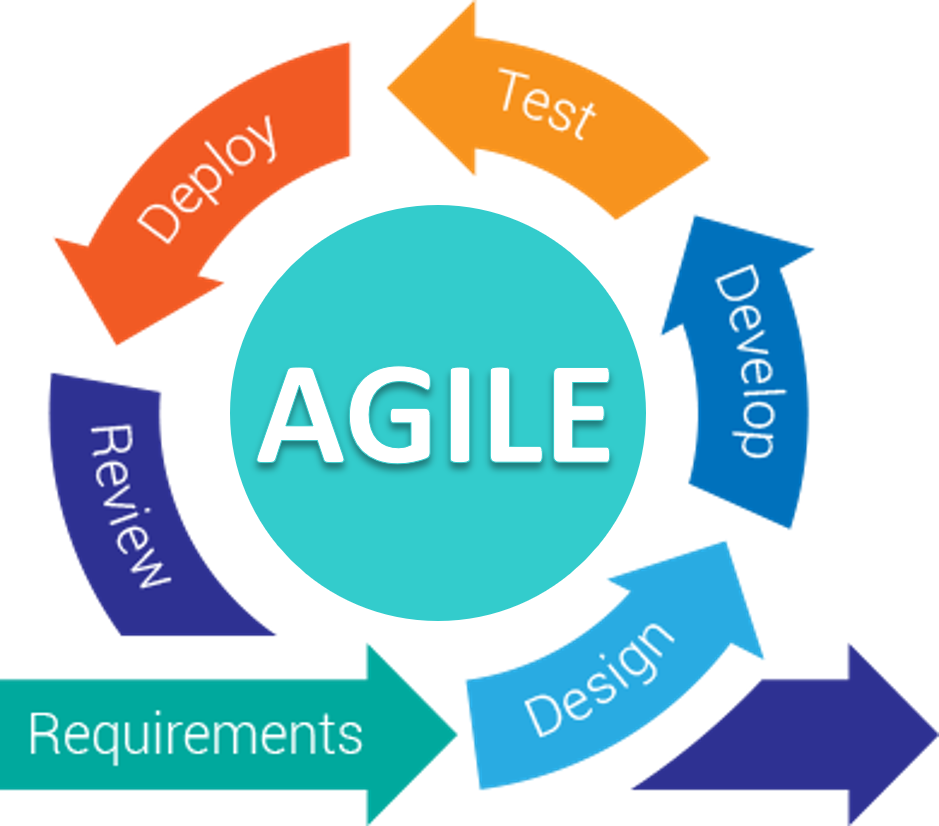
\includegraphics[width= 3in ]{agile.png}
%     \caption{Agile Model}
% \end{figure}




\begingroup

\let\clearpage\relax
\subsection{System Development Tools}
Our static Deepfake detection System requires Python, Tensorflow, OpenCV,
Machine Learning which are listed below:
\begin{enumerate}
    \item Python
    \item Pytorch
    \item NumPy
    \item OpenCV
\end{enumerate}


\subsection{Functional Requirement}
The functional requirements of the system are:
\begin{enumerate}
    \item Authentication of users.
    \item User-friendly interface for uploading and detection.
    \item Image preprocessing.
    \item Mathematical Modeling and Implication. 
    \item Model Development and training.
    \item Testing and Validation.

\end{enumerate}
\subsection{Non Functional Requirement}
\justify
These requirements are not needed by the system but are essential for the better
performance of software. The points below focus on the non-functional requirement of
the system.
\begin{itemize}
    \item Reliability
    \item   Usability
    \item   Security
    \item   Portability
    \item   Speed and responsiveness
    \item  Performance
\end{itemize}

\endgroup

\newpage


\section{SYSTEM ARCHITECTURE AND METHODOLOGY }
\subsection{Block Diagram}
\begin{figure}[h]
    \centering
    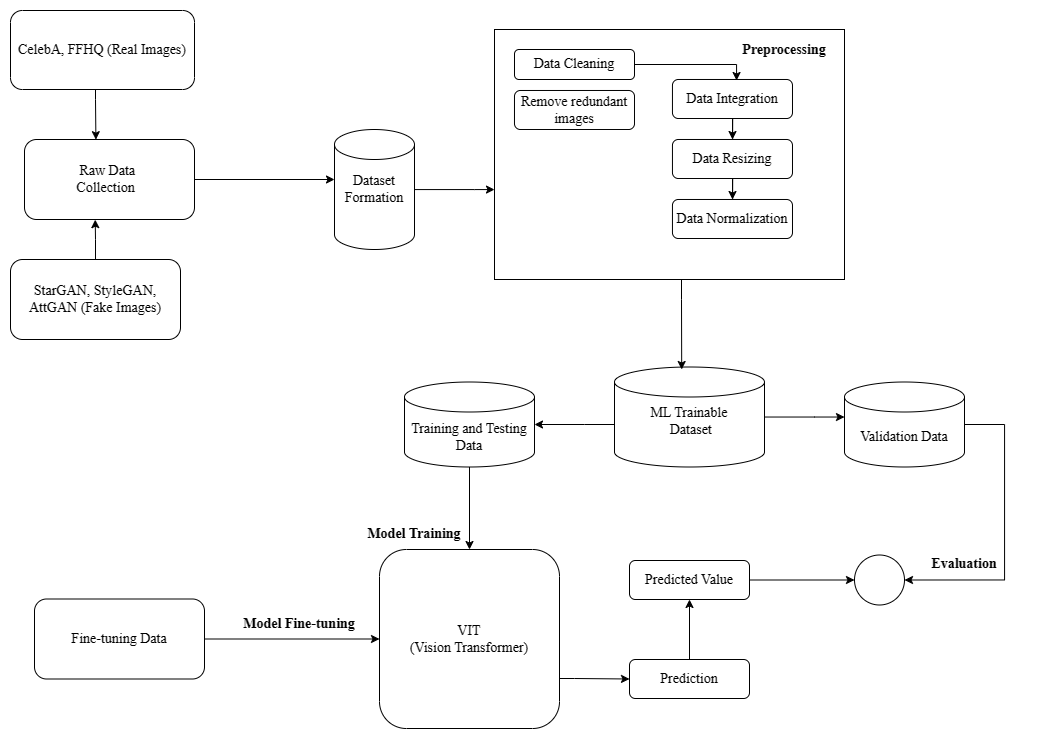
\includegraphics[width= 6.5in ]{img/Model_Architecture.drawio (4).png}
    \caption{{System Architecture}}

\end{figure}
\justify
The system architecture of our project involves multiple steps. Initially, the formation of datasets takes place as raw data are collected to training, testing and validation  The frames are extracted from the input video or obtained directly from an image. These frames then undergo face extraction, where faces are identified and cropped using face detection algorithms. The extracted faces are resized to a standardized size and undergo normalization to ensure consistent pixel values. The preprocessed face images are then fed into a deep learning model for classification. The model analyzes the features and patterns in the images to determine whether they are real or fake. Finally, the system produces the output, indicating the authenticity of the input video or image as either real or fake.

\newpage



\subsection{Use Case Diagram}
\begin{figure}[h]
    \centering
    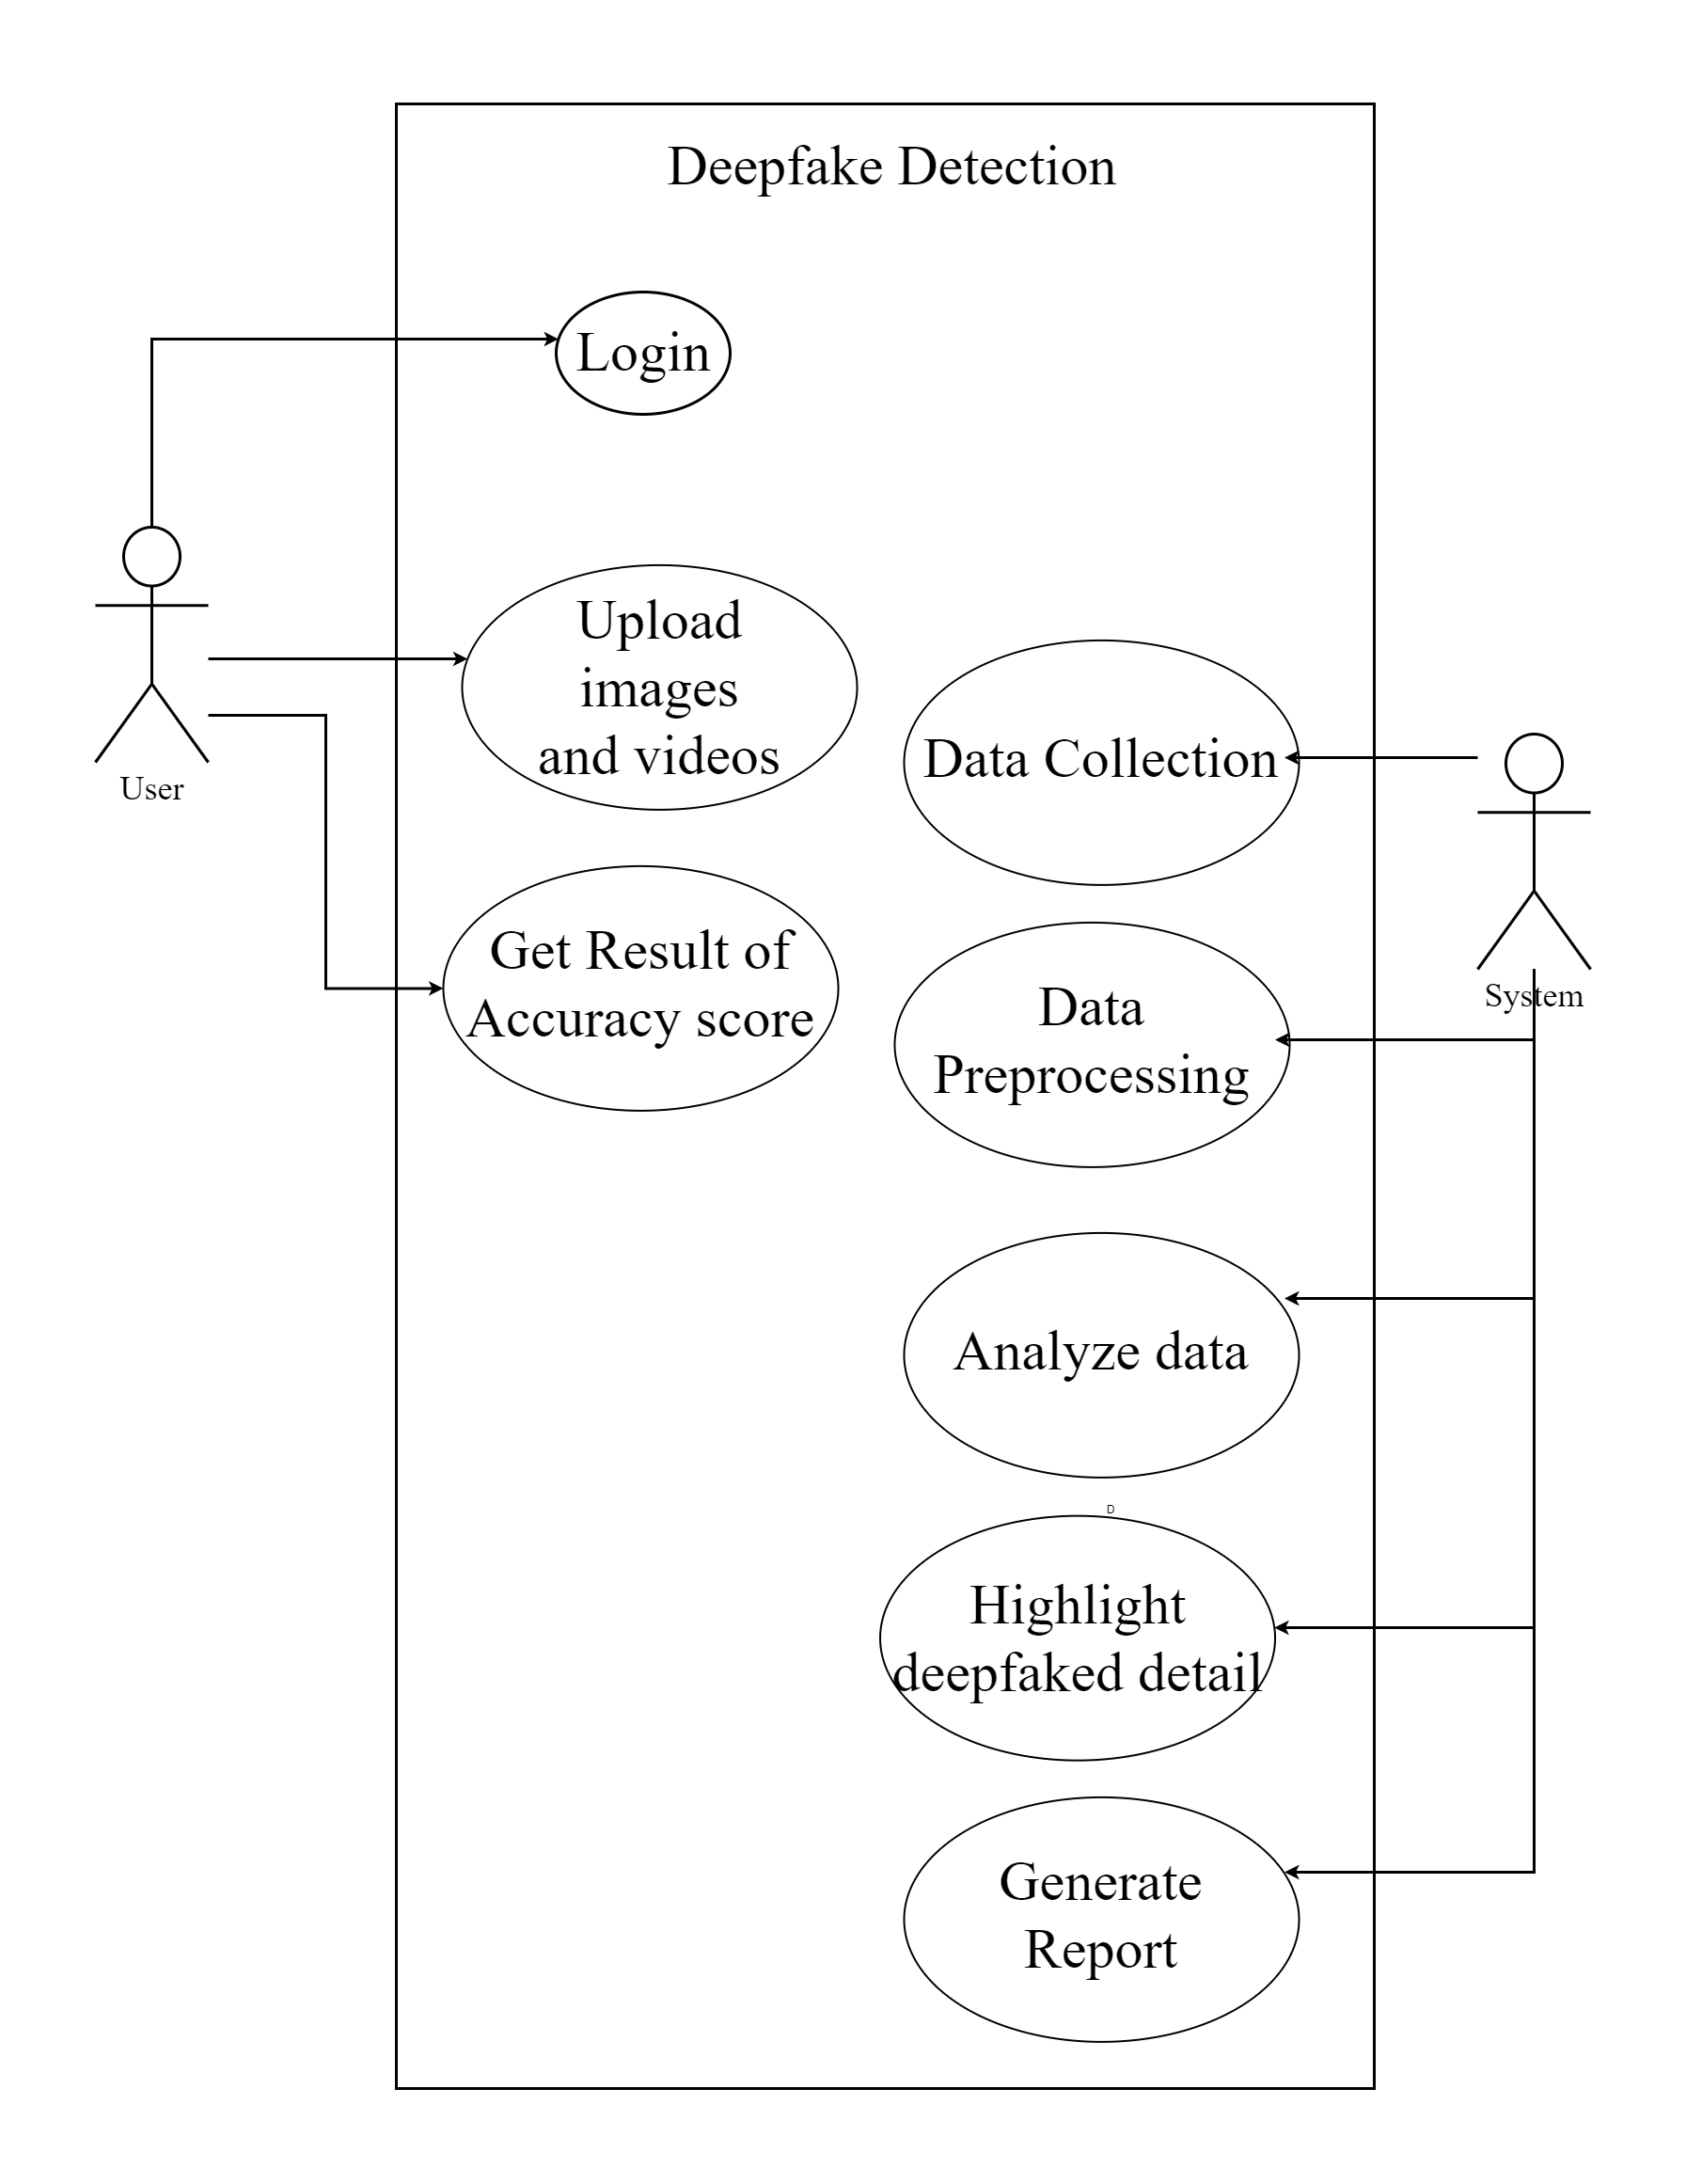
\includegraphics[width= 5.5in ]{img/usecasediagram.drawio.png}
    \caption{{Use Case Diagram}}
\end{figure}
\justify
The use case diagram for our system illustrates various interactions and roles of the system's users. The primary actors involved are the "User" and the "System." The User interacts with the system by initiating the deepfake detection process, either by uploading a video or an image. The User can also access the system to view the detection results. On the other hand, the System is responsible for managing the system, including user authentication, system configuration, and monitoring the overall functionality. The use case diagram shows the main use cases, such as "Upload Media," "Detect Deepfake," and "View Results," which represent the key functionalities of the system.
\newpage


\subsection{Sequence Diagram}

\begin{figure}[h]
    \centering
    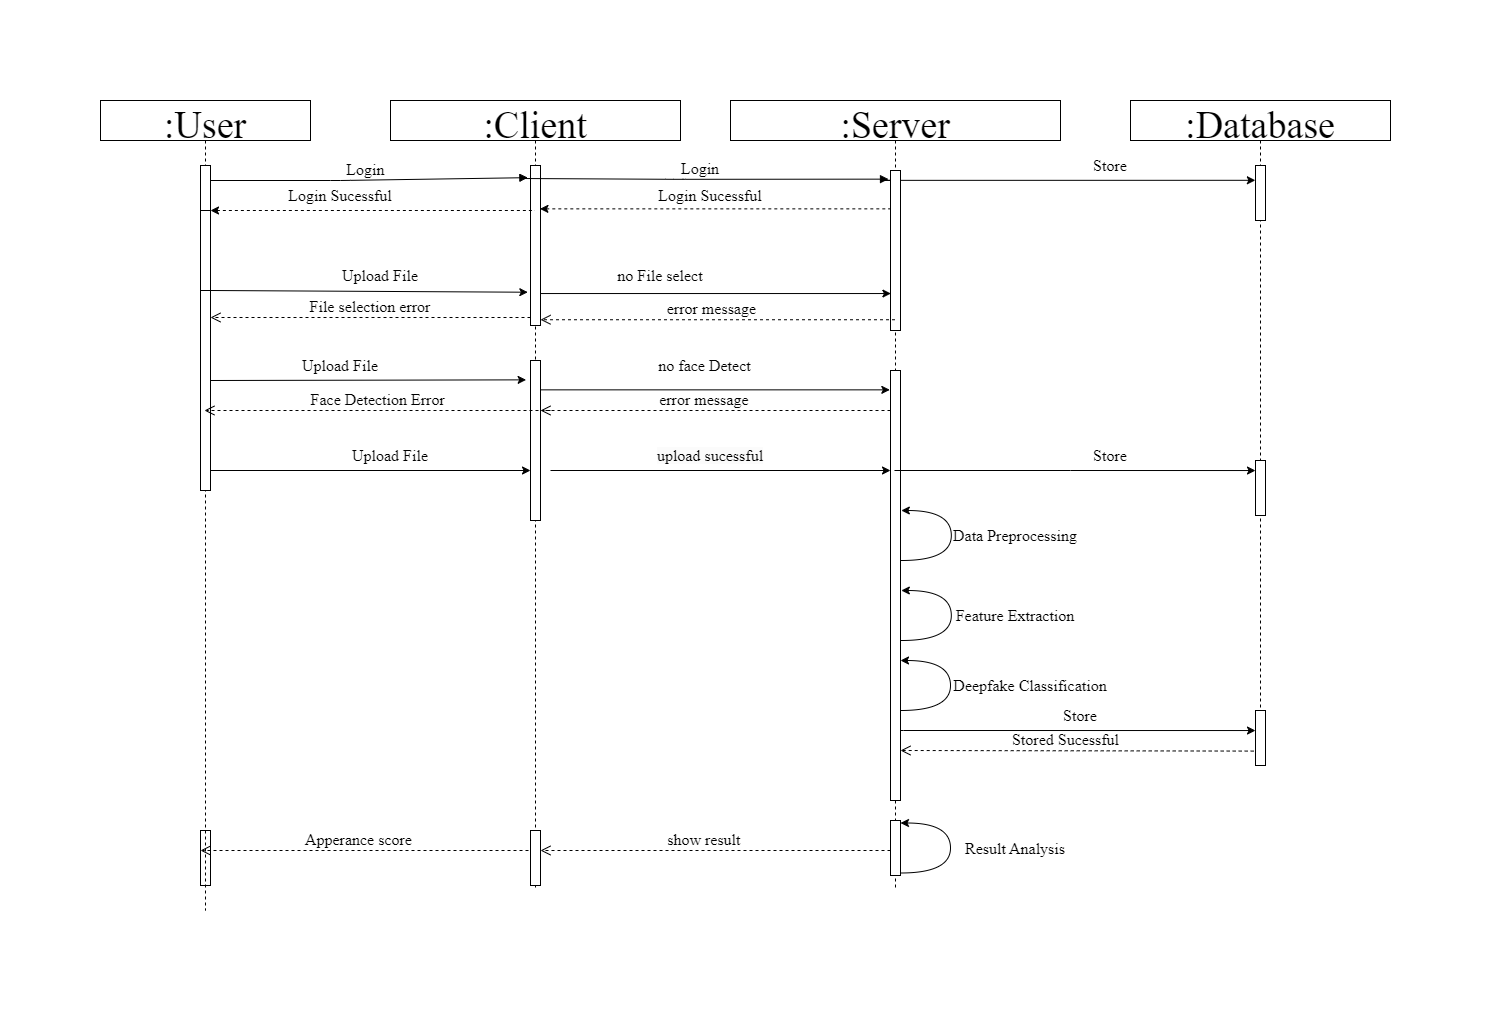
\includegraphics[width=8in]{img/sequencediagram.drawio.png}
    \caption{\textit{Sequence Diagram}}
\end{figure}

\justify
The sequence diagram shows that the user initiates the process by accessing the system and providing their login credentials. The Server checks the login credentials and verifies the user's identity. Once authenticated, the user proceeds to upload a file containing the video or image to be analyzed for deepfakes. Then face detection algorithms are used to detect and extract faces from the uploaded media. This collected data undergoes further processing, including resizing and normalization, to prepare it for deep learning modeling. Finally, the processed data is fed into the deep learning model, which analyzes the features and patterns to classify the media as either real or fake.



\subsection{Dataflow Diagram}
\begin{figure}[h]
    \centering
    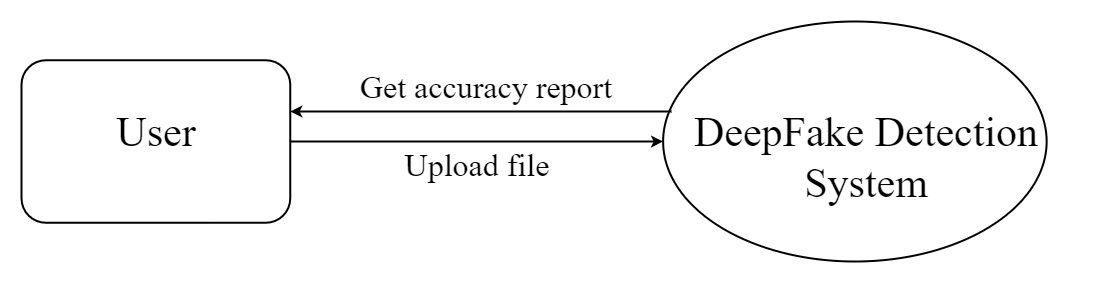
\includegraphics[width= 4in ]{img/level0dfd.drawio.png}
    \caption{\textit{Level 0 DFD}}
\end{figure}

\justify
DFD level – 0 indicates the basic flow of data in the system.
\begin{itemize}
    \item User: User input to the system is uploading video.
    \item System: In system it shows all the details of the Video and output shows the fake video or not. \\
          and output flow
\end{itemize}
Hence, the data flow diagram indicates the visualization of system with its input feed to the system by User.\\
\begin{figure}[h]
    \centering
    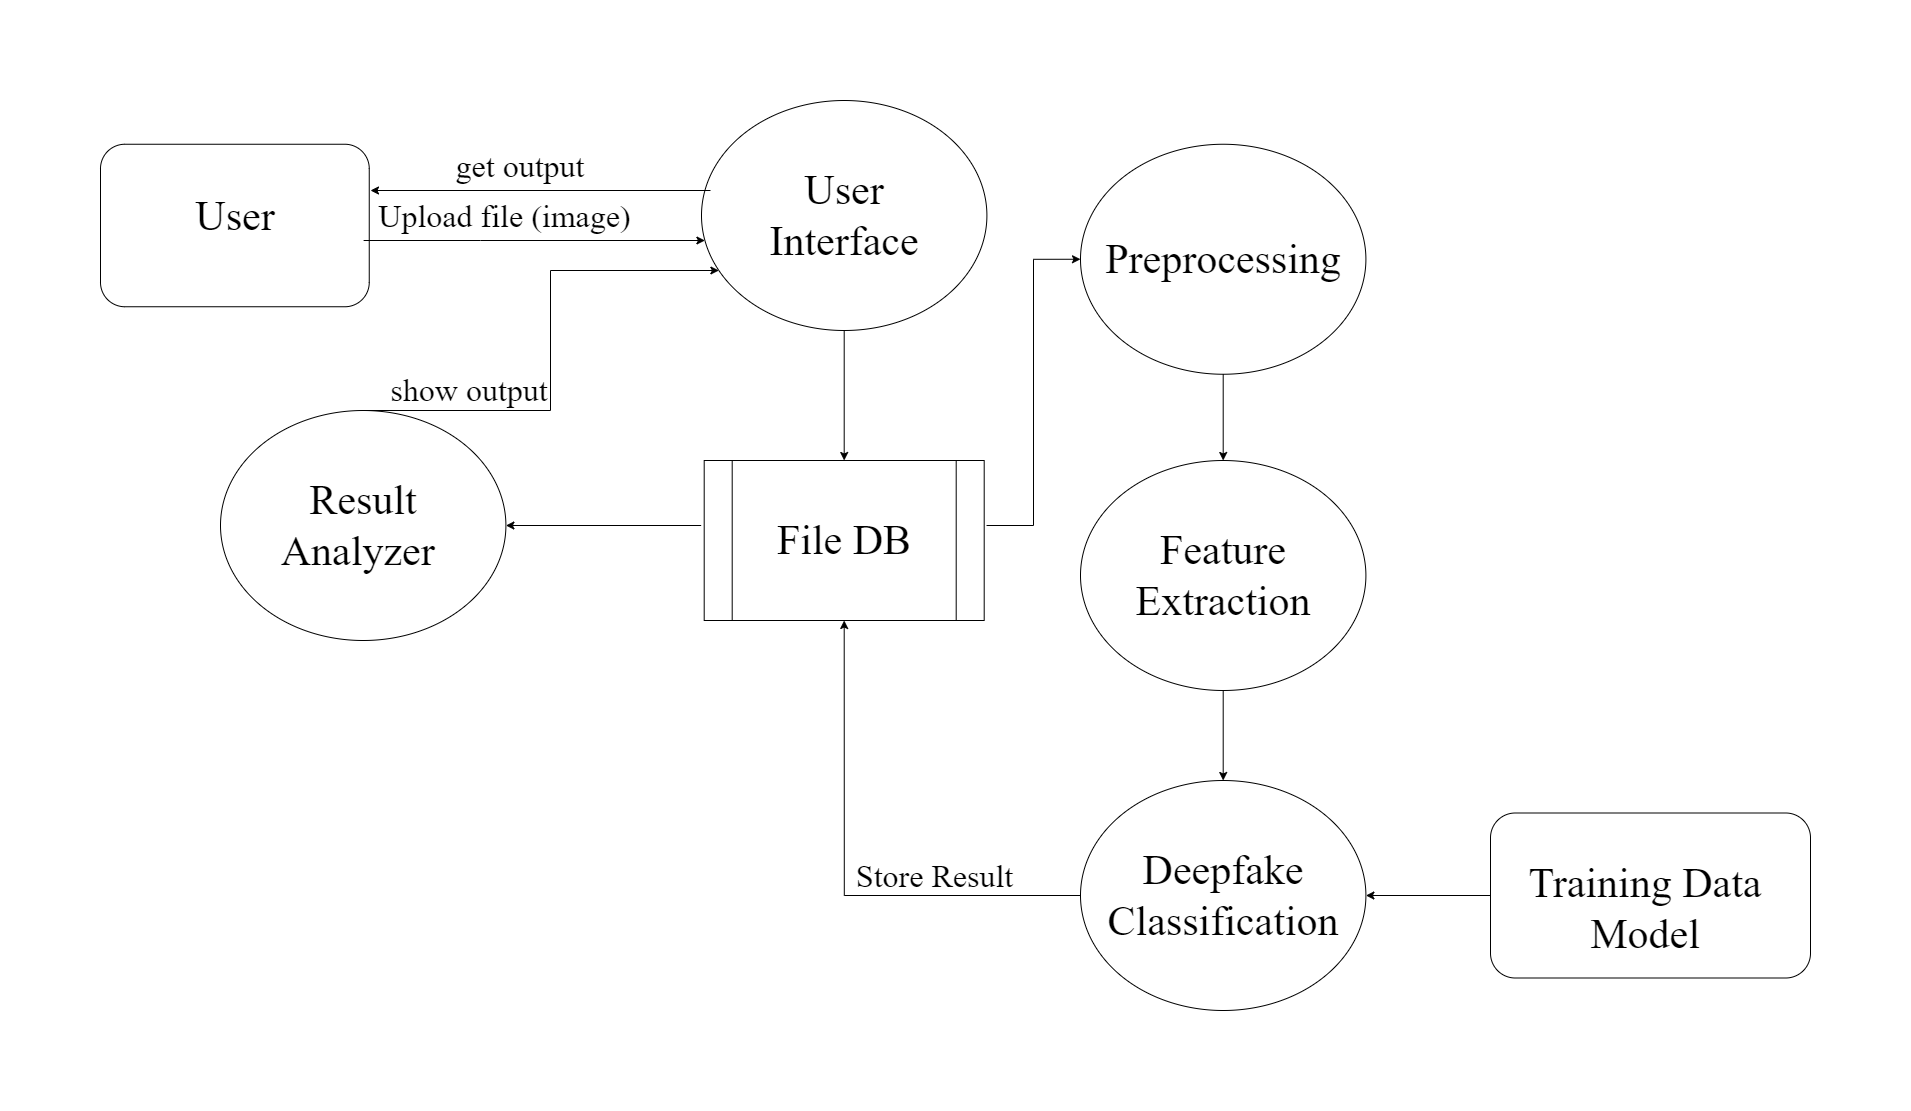
\includegraphics[width= 6in ]{img/level1dfd.drawio.png}
    \caption{\textit{Level 1 DFD}}
\end{figure}
\justify
DFD Level – 1 gives more in and out information of the system.Where system gives detailed information of the procedure taking place.



\subsection{Activity Diagram}
\newpage



\section{CONCLUSION}
 In summary, our project for spotting fake media using Vision Transformers is a strong and easy-to-use solution. The simple interface makes it easy for users to upload content and see results clearly. Our system is really efficient and effective for detection of manipulated contents, with an impressive average accuracy of about 92.85\% in different tests. It stays strong against real-bound images and tackle attacks, proving its reliability even in tough situations. By using recent tools and technology, a straightforward interface, and being strong against different manipulative contents, our project becomes a useful tool in stopping the spread of fake graphical media online.
\newpage




% \section{LIMITATIONS}
% \begin{itemize}
%     \item Deepfake detection projects face challenges due to rapidly evolving techniques and the need for diverse training data.
%     \item Adversarial attacks can exploit weaknesses in detection algorithms, making deepfakes harder to identify accurately.
%     \item Deepfake detection algorithms often require significant computational resources, limiting their applicability on resource-constrained devices.
% \end{itemize}
\newpage


% \section{FUTURE ENHANCEMENTS}
% There is always a scope for enhancements in any developed system, especially
% when the project build using latest trending technology and has a good scope in
% future.
% \begin{itemize}
%     \item Web based platform can be upscaled to a browser plugin for ease of access to
%           the user.
%     \item Currently only Face Deep Fakes are being detected by the algorithm, but the
%           algorithm can be enhanced in detecting full body deep fakes.
% \end{itemize}

\newpage


\begin{thebibliography}{99}

    \bibitem{1} Andreas Rossler, Davide Cozzolino, Luisa Verdoliva, Christian Riess, Justus Thies, Matthias Nießner, "FaceForensics++: Learning to Detect Manipulated Facial Images"

    % \bibitem{2} Deepfake detection challenge dataset: \url{https://www.kaggle.com/c/deepfake-detection-challenge/data}

    % \bibitem{3} Yuezun Li, Xin Yang, Pu Sun, Honggang Qi, and Siwei Lyu, "Celeb-DF: A Large-scale Challenging Dataset for DeepFake Forensics"

    % \bibitem{4} "10 deepfake examples that terrified and amused the internet," Creative Bloq, \url{https://www.creativebloq.com/features/deepfake-examples}

    % \bibitem{5} Keras, \url{https://keras.io/}

    % \bibitem{6} PyTorch, \url{https://pytorch.org/}

    % \bibitem{7} G. Antipov, M. Baccouche, and J.-L. Dugelay, "Face aging with conditional generative adversarial networks"

    % \bibitem{8} TensorFlow, \url{https://www.tensorflow.org/}

    % \bibitem{9} FaceApp, \url{https://www.faceapp.com/}

    % \bibitem{10} Face Swap, \url{https://faceswaponline.com/}
    \bibitem{2} iproov, "How To Protect Against Deepfakes – Statistics and Solutions" (2022). \url{https://www.iproov.com/blog/deepfakes-statistics-solutions-biometric-protection}
    \bibitem{3} Douglas Blakey, "Forced verification and AI/deepfake cases multiply at alarming rates: Sumsub" (2023). \url{https://www.electronicpaymentsinternational.com/news/forced-verification-and-ai-deepfake-caeses-sumsub/}
    \bibitem{4} C. Vaccari and A. Chadwick, “Deepfakes and disinformation: exploring the impact of synthetic political video on deception, uncertainty, and trust in news,” Social Media+ Society, vol. 6, no. 1, p.2056305120903408, 2020
    
    \bibitem{5} X. Zhang, S. Karaman, and S.-F. Chang, “Detecting and simulating artifacts in gan fake images,” in 2019 IEEE International Workshop on Information Forensics and Security (WIFS). IEEE, 2019, pp. 1–6. 1, 3, 10
    
    \bibitem{6}  L. Guarnera, O. Giudice, C. Nastasi, and S. Battiato, “Preliminary forensics analysis of deepfake images,” in 2020 AEIT International Annual Conference (AEIT), 2020, pp. 1–6. 1, 7
    
    \bibitem{7}R. Durall, M. Keuper, F.-J. Pfreundt, and J. Keuper, “Unmasking deepfakes with simple features,” arXiv preprint arXiv:1911.00686, 2019.
    \bibitem{8} Han, K., Xiao, A., Wu, E., Guo, J., XU, C., and Wang, Y. (2021). "Transformer in Transformer".
    \bibitem{9} Dosovitskiy, A., Beyer, L., Kolesnikov, A., Weissenborn, D., Zhai, X., Unterthiner, T., Dehghani, M., Minderer, M., Heigold, G., Gelly, S., Uszkoreit, J., and Houlsby, N. (2021). "An Image is Worth 16x16 Words: Transformers for Image Recognition at Scale. In International Conference on Learning Representations"
    \bibitem{10} Y. Liu et al., "A Survey of Visual Transformers," in IEEE Transactions on Neural Networks and Learning Systems.
    


    \bibitem{11} Yang Liu, Yao Zhang, Yixin Wang, Feng Hou, Jin Yuan,
    Jiang Tian, Yang Zhang, Zhongchao Shi, Jianping Fan, Zhiqiang He. (2021). "A Survey of Visual Transformers".

    \bibitem{12} Vaswani, A., Shazeer, N., Parmar, N., Uszkoreit, J., Jones, L., Gomez, A. N. and Polosukhin, I. (2017). "Attention is all you need. In Advances in neural information processing systems (Vol. 30)".
    \bibitem{22}B. Bahmei, E. Birmingham and S. Arzanpour, "CNN-RNN and Data Augmentation Using Deep Convolutional Generative Adversarial Network for Environmental Sound Classification," in IEEE Signal Processing Letters, vol. 29, pp. 682-686, 2022, doi: 10.1109/LSP.2022.3150258.


\end{thebibliography}

\end{document}